\documentclass{standalone}
\usepackage{tikz}

\begin{document}

\centering

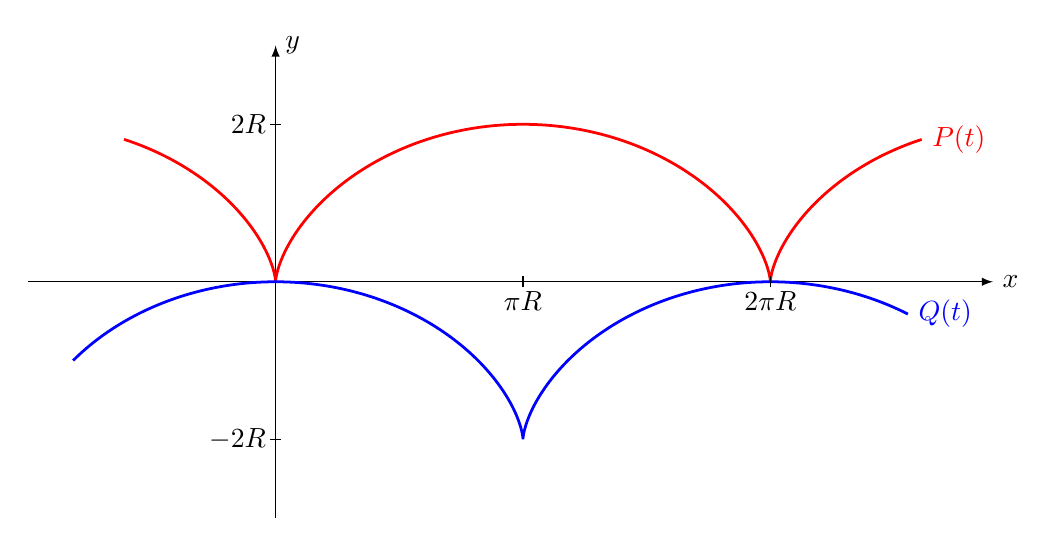
\begin{tikzpicture}
    % draw axes
    \coordinate (O) at (0,0);
    \draw[-latex] (0,-3) -- (0,3) node[anchor=west] {$y$};
    \draw[-latex] (-pi,0) -- (2.9*pi,0) node[anchor=west] {$x$};

    % draw cycloid
    \def\r{1} % radiusdsf
    \draw[red,domain=-0.8*pi:2.8*pi,samples=200, line width=1, smooth] plot ({\x - sin(\x r)},{1 - cos(\x r)}) node[right] {$P(t)$}; 
    % \x r means to convert '\x' from degrees to radians

    \draw[blue,domain=-0.5*pi:2.3*pi,samples=200, line width=1, smooth] plot ({\x + sin(\x r)},{-1 + cos(\x r)}) node[right] {$Q(t)$}; 
    
    

    % labels x-axis
    \node[anchor=north] at (2*pi,0) {$2 \pi R $};
    \node[anchor=north] at (pi,0) {$\pi R $};
    \draw (pi,-2pt) -- (pi,2pt);
    \draw (2*pi,-2pt) -- (2*pi,2pt);

    % labels y-axis
    \node[anchor=east] at (0,2) {$2R $};
    \node[anchor=east] at (0,-2) {$-2R$};
    \draw (-2pt,2) -- (2pt,2);
    \draw (-2pt,-2) -- (2pt,-2);
        
\end{tikzpicture}
\end{document}